\documentclass[titlepage, 12pt]{article}
\usepackage[parfill]{parskip}
\usepackage{xcolor}
\usepackage{setspace}
\usepackage{hyperref}
\usepackage[T1]{fontenc}
\usepackage[utf8]{inputenc}
\usepackage{graphicx}
\graphicspath{ {./assets/} }

\usepackage{charter}

\hypersetup{
    colorlinks=true,
    linkcolor=blue,
    filecolor=magenta,
    urlcolor=blue,
}

\begin{document}

\begin{titlepage}

	\raggedleft

	\vspace*{\baselineskip}

	{Bharathi Ramana Joshi 2019121006\\Jayati Narang 2018101066}

	\vspace*{0.167\textheight}

	\textbf{\Large Project proposal for}\\[\baselineskip]

	\textbf{\textcolor{teal}{\huge Data visualization}}\\[\baselineskip]

    {\large \textit{Team: namesarehard}}
    \vfill

    \today

	\raggedright

\end{titlepage}

\newpage

\tableofcontents

\newpage

\section{Introduction}

\subsection{Why use Visualization?}
Quoting the definition of data visualization from Munzner,
\begin{quotation}
    ``Computer-based visualization systems provide visual representations of
    datasets designed to help people carry out tasks effectively - i.e. vis
    systems are appropriate for use when your goal is to augment human
    capabilities, rather than completely replace the human in the loop\dots''
\end{quotation}
Therefore, we first came up with a set of interesting questions related to the
dataset and then we came up with intuitive solutions to these questions that use
data visualization.

\subsection{The dataset being used}
After browsing through a plethora of datasets, we finally decided to go with
\href{https://www.kaggle.com/uciml/student-alcohol-consumption/data}{Student
Alcohol Consumption}. Our reasons for selecting this particular dataset over
others were
\begin{enumerate}

    \item It had 31 diverse fields, enabling us to ask numerous intriguing
        questions.

    \item The values in the lion's share of the fields were well distributed,
        unlike other datasets where several fields had clustered values. This
        made visualization an appropriate tool to augment human rationality to
        answer questions related to the dataset.

    \item We felt the dataset's theme and, consequently the questions, were
        quite pertinent to our day to day lives as it is an unspoken truth that
        many of our peers indulge in drinking.

\end{enumerate}

\subsection{The datasets not being used}
Some datasets that we did \textbf{not} use after considerable inspection are
\begin{enumerate}

    \item\href{https://www.kaggle.com/osmi/mental-health-in-tech-survey}{Mental
        Health in Tech Survey} - although this had copious fields, the values in
        each field were clustered, making visualization an overkill solution for
        any questions we could ask about the dataset.

    \item\href{https://www.kaggle.com/datasnaek/chess}{Chess Game Dataset
        (Lichess)} - despite the fact that this dataset was quite apt as one of
        our team members is a chess aficionado,
        \href{https://lichess.org/}{Lichess} already provides
        \href{https://lichess.org/blog/VmZbaigAABACtXQC/chess-insights}{Chess
        Insights}, which we were sure we couldn't beat. We highly recommend the
        reader to go through Chess Insights for a
        \href{https://lichess.org/insights/The_Mockingbird/acpl/variant}{Lichess
        user} for some truly marvellous applications of data visualization.

    \item\href{https://github.com/covid19india/api}{covid19india} - given the
        current circumstances, this is perhaps the most relevant dataset.
        However, we knew that many other teams were using this and it would be
        difficult for us to stand out if we were also to use this dataset. Thus
        we decided against it.

\end{enumerate}
We feel these were worth mentioning as we spent a significant amount of time
scrutinizing these.

\section{Questions and Visualizations}
Although the data was surveyed primarily to study students' alcohol consumption,
we realized that myriads of questions could be asked that aren't related to
this, and that is exactly what we ended up doing.

On a side note, we request the reader to go through at least the Description
section on the
\href{https://www.kaggle.com/uciml/student-alcohol-consumption}{dataset's Kaggle
page} before proceeding further.
\subsection{Parents' education and employment vs support}
We've decided to use parallel sets to answer this question - the axes will be
parent's education, employment and educational support provided, in that
specific order. There will also be a radio button / drop down selection for
selecting between the parents. A rough sketch is as follows

\begin{center}
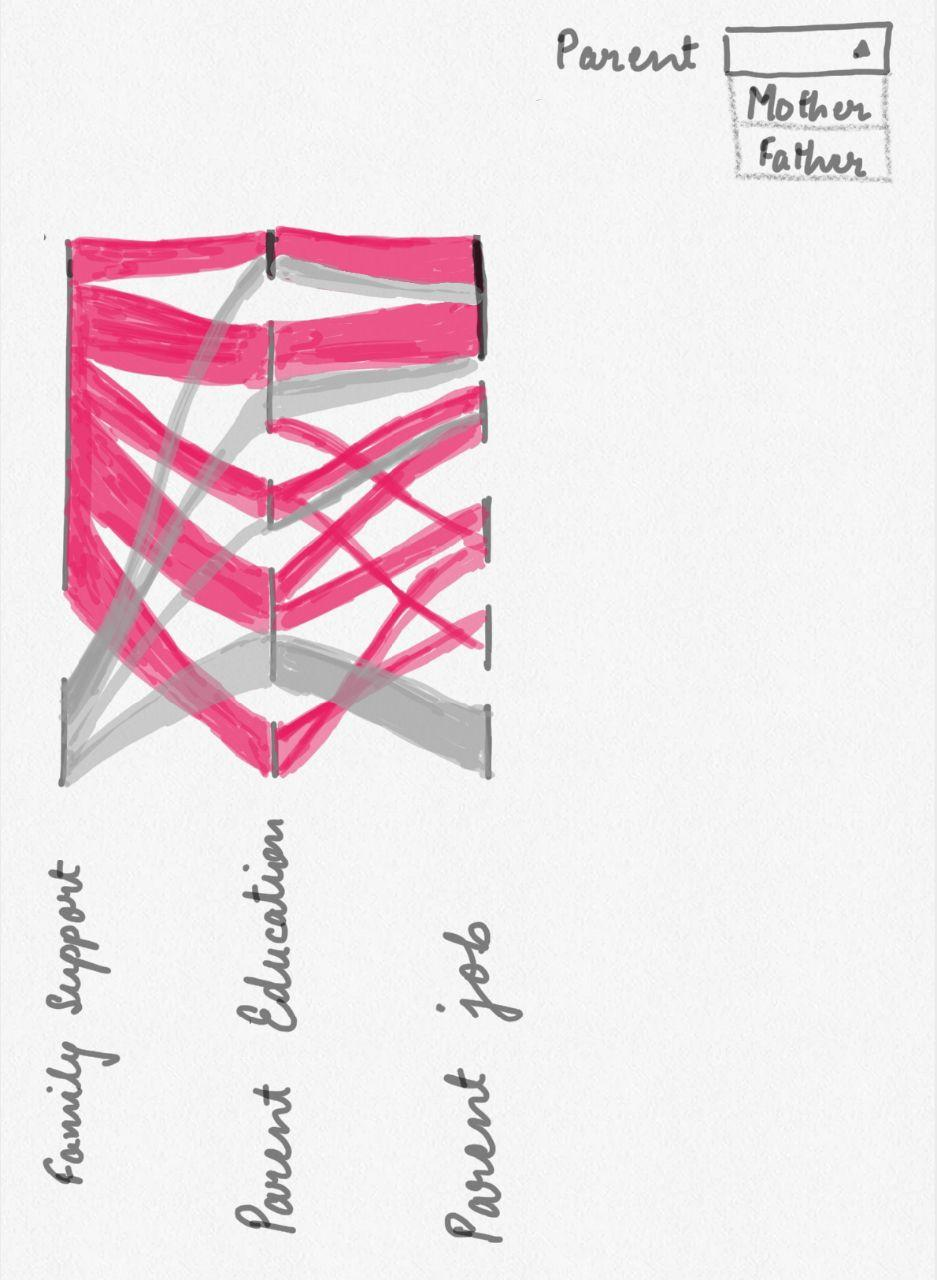
\includegraphics[scale=0.3]{1}
\end{center}

\subsection{Relevant binary field vs alcohol consumption}
A few relevant binary fields we identified were relationship status, sex,
school's educational support and family's educational support.  After careful
consideration, we've concluded that a pie chart will be the most effective
visualization here. The binary field (first axis) will partition the entire data
set into two separate sets, which will be visualized using two different colors.
We will then use different gradients of these two colors to differentiate
between different levels of alcohol consumption. A rough sketch is as follows

\begin{center}
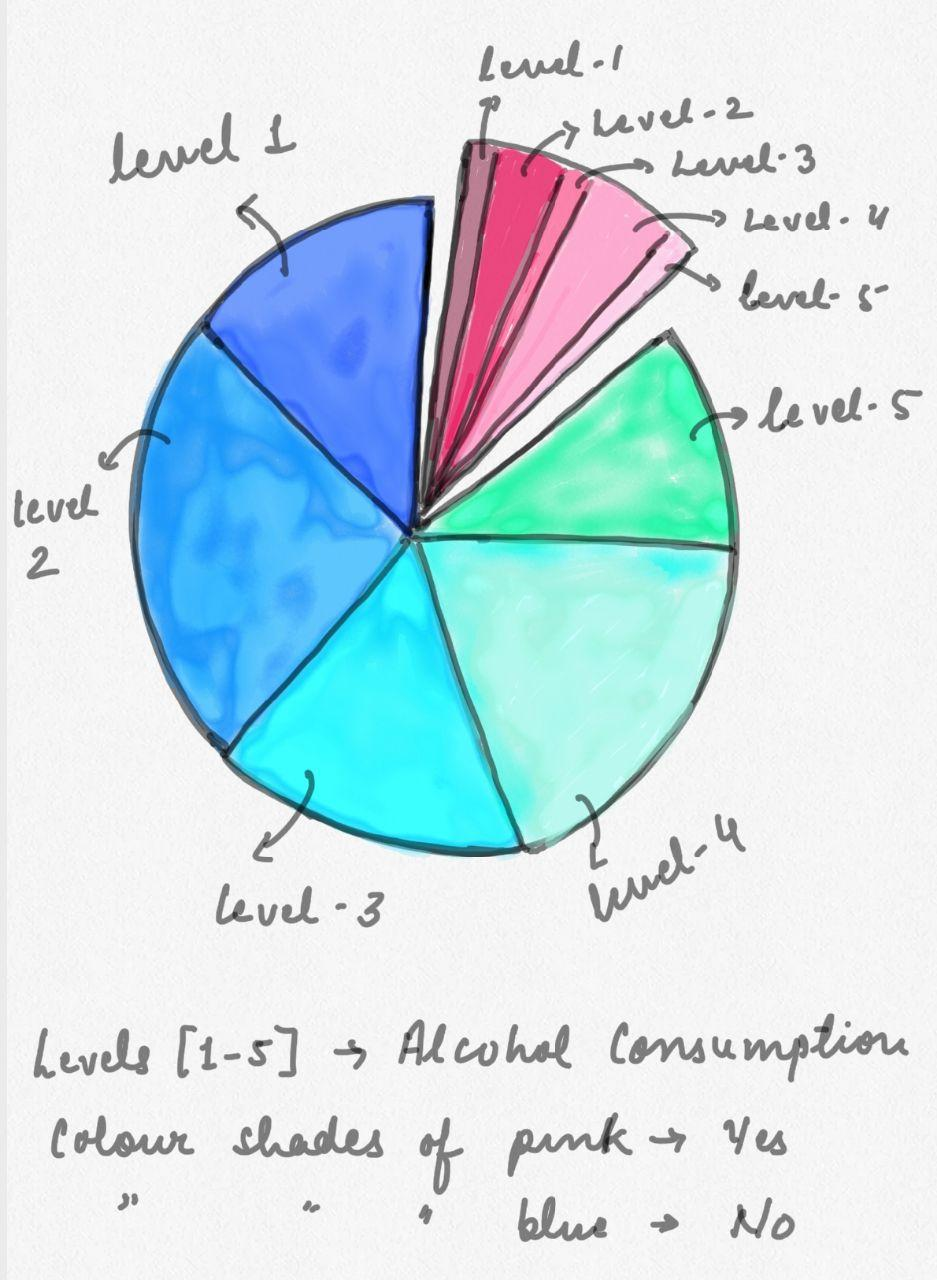
\includegraphics[scale=0.3]{2}
\end{center}

\subsection{Study time vs grades}
A contour will succinctly visualize this. Study time on X-axis and failures
on Y-axis will be measured. Intensity of color at a point will denote number of
students there. A rough sketch is as follows

\begin{center}
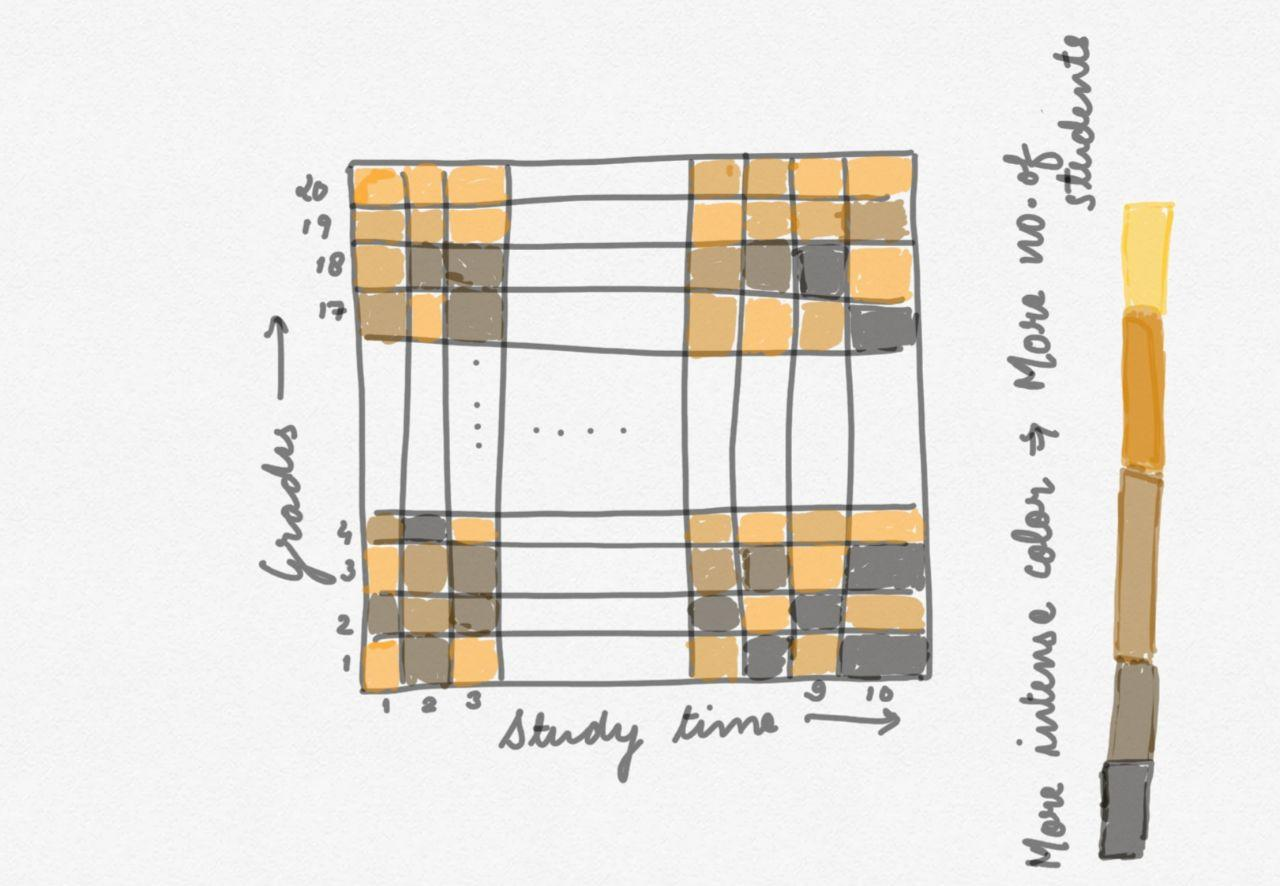
\includegraphics[scale=0.3]{3}
\end{center}

\subsection{Ages, going out vs alcohol consumption}
Scrutinizing led us to deduce that a bubble chart is well suited to visualizing
this question. The X-axis will measure age, Y-axis degree of going out with
friends and size of circle amount of alcohol consumed. Furthermore, we plan to
distinguish weekend and weekday alcohol consumption by either using bubbles of
different colors (and plot them in the same graph) or providing a button for
selection (and plot them separately). Rough sketch is as follows

\begin{center}
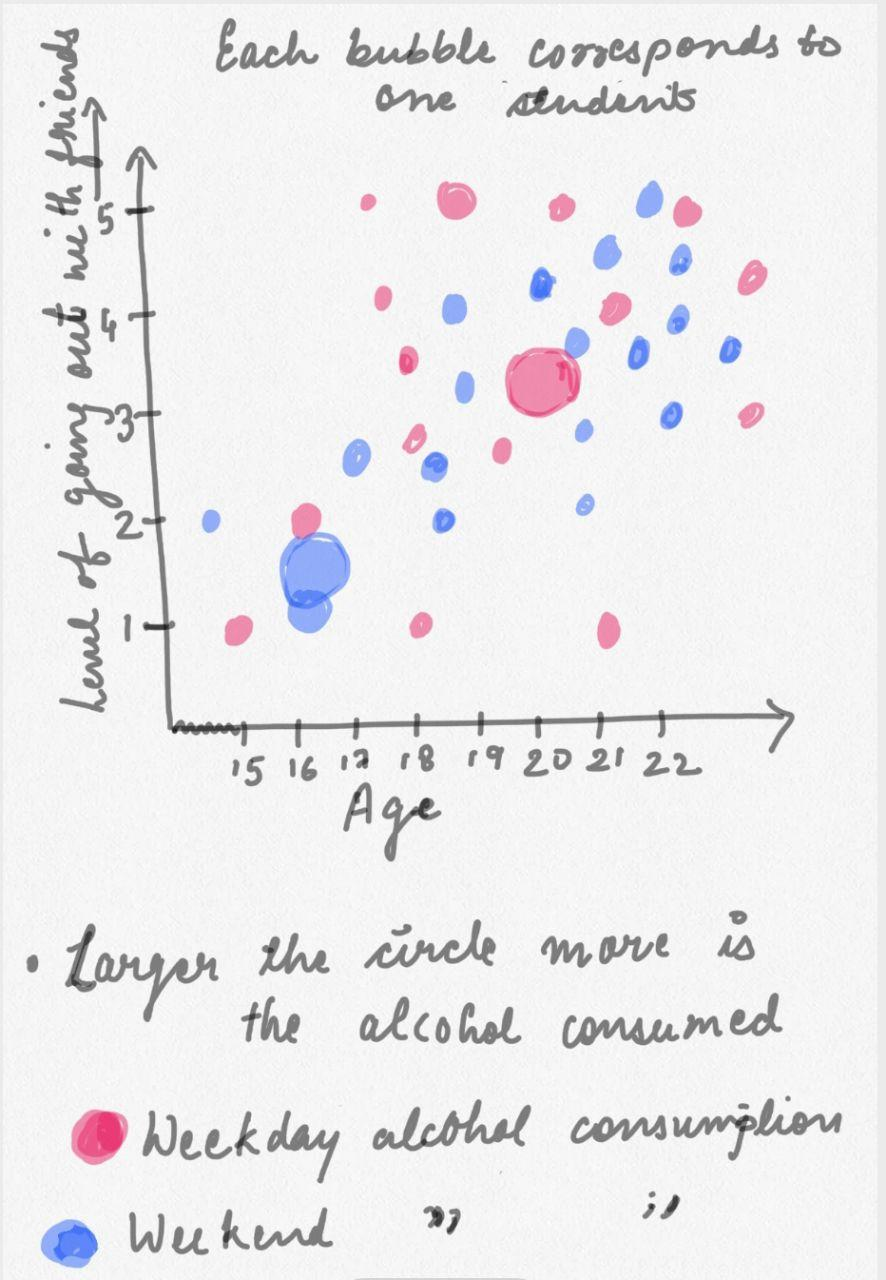
\includegraphics[scale=0.3]{4}
\end{center}

\subsection{Absences, parents' habitation status vs avg. failures}
A steam graph is apt for this visualization. The X-axis will denote absences,
Y-axis failures and colors to distinguish between parents' cohabition status. If
feasible, we plan to provide a drop down / radio button selection of measure of
central tendency. Rough sketch is as follows

\begin{center}
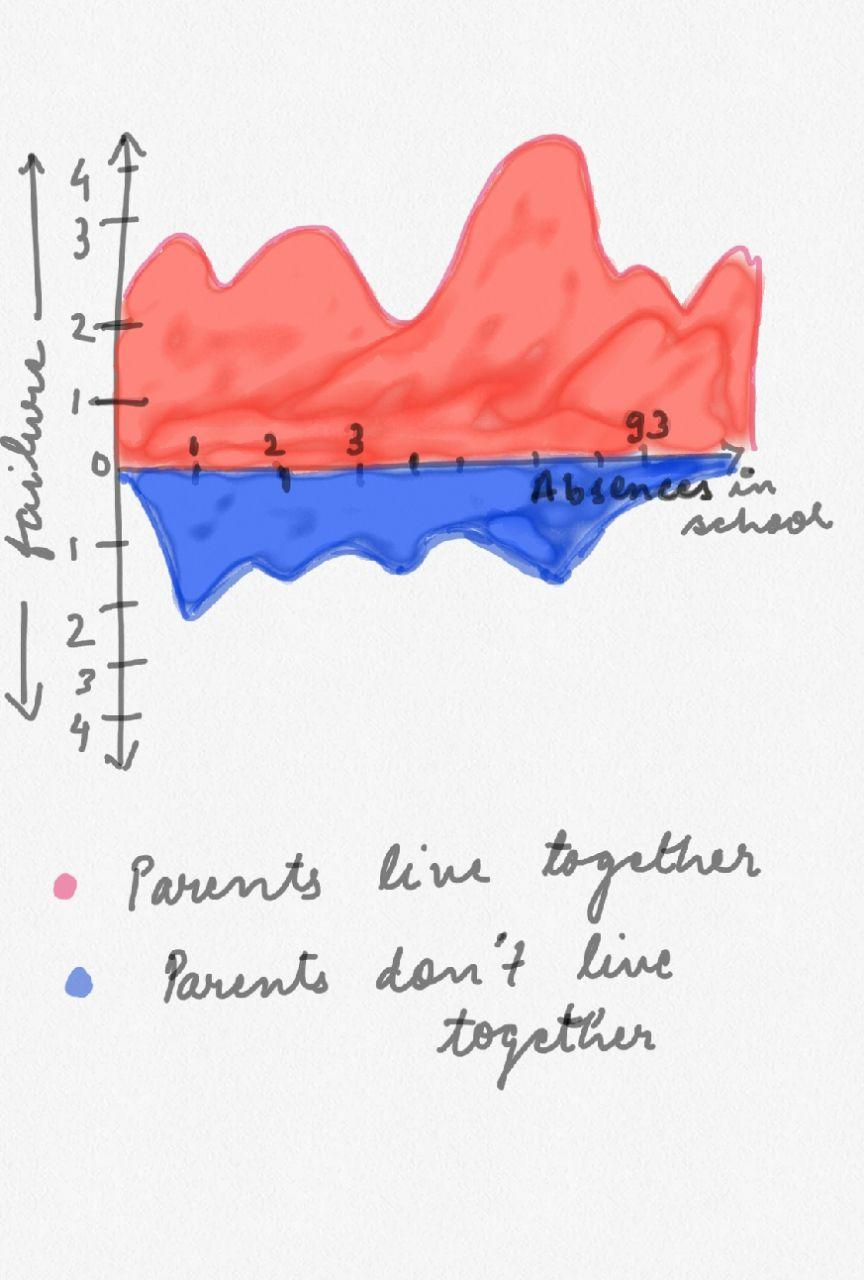
\includegraphics[scale=0.3]{5}
\end{center}

\subsection{Health vs alcohol consumption}
A scatter plot visualization is fitting here. X-axis will denote health and
Y-axis alcohol consumption. Colors will be used to distinguish between weekend
and weekday consumption. Intensity of color will indicate population. Rough
sketch is as follows

\begin{center}
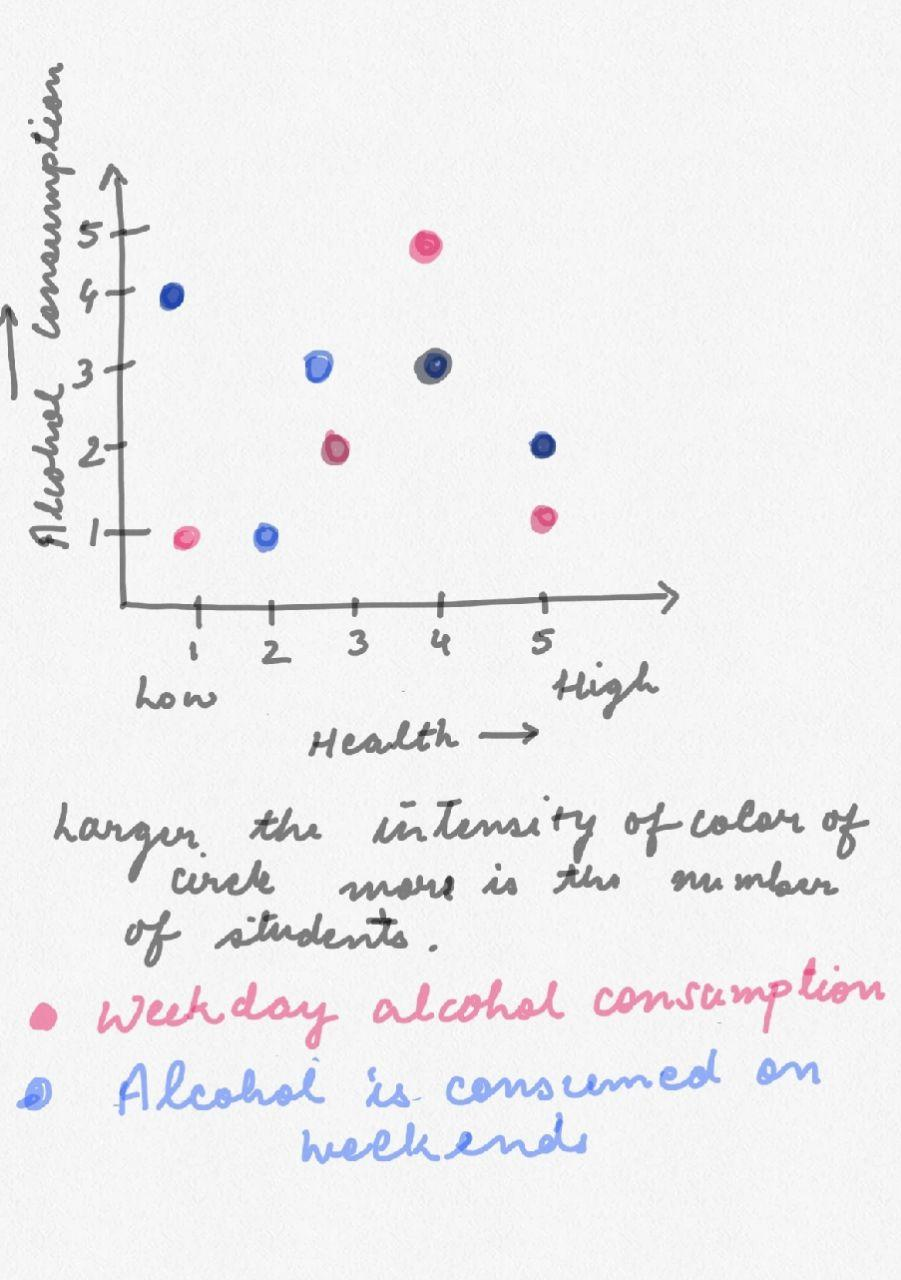
\includegraphics[scale=0.3]{6}
\end{center}

\subsection{Study time vs failures}
A heat map using a pairwise correlation matrix is the favourable to answer this
question. X-axis will denoted study time, Y-axis failures and intensity of color
the number of students in that category. This will look similar to 2.3.

\subsection{Family size, relationships' quality vs alcohol consumption}
A stacked bar chart will be appropriate for this question. X-axis will denote
alcohol consumption, Y-axis quality of relationships and two different colors
will differentiate between different family sizes. A radio button / drop down
menu will be used to distinguish between weekend and weekday consumption. Once
again, if feasible, we plan to provide a drop down / radio button selection of
measure of central tendency. Rough sketch is as follows

\begin{center}
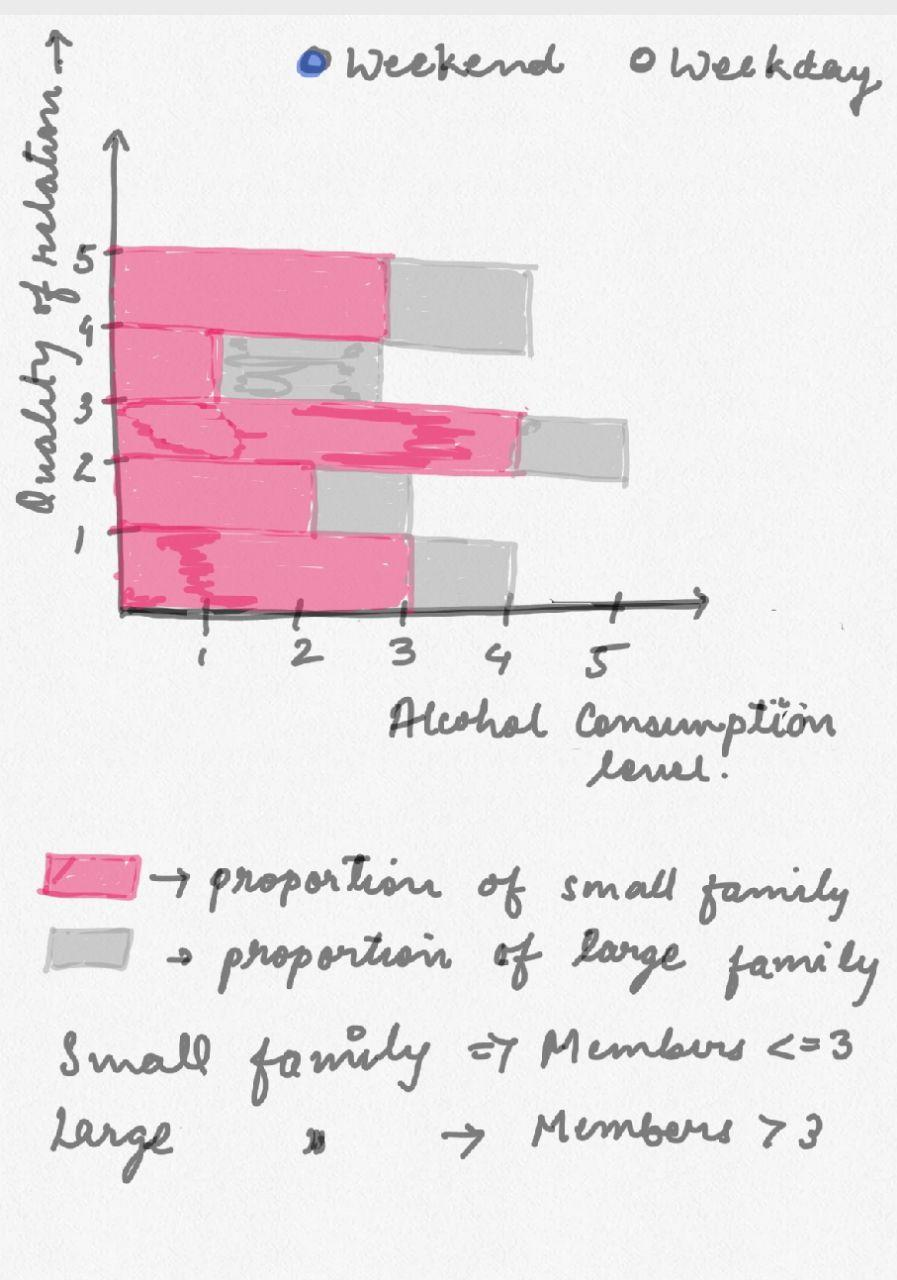
\includegraphics[scale=0.3]{8}
\end{center}

\end{document}
